\documentclass[]{report}
\usepackage{amsmath,amsfonts,graphicx}

\def\species{\mathrm{sp}}
\def\phase{\mathrm{ph}}
\def\massfrac{\chi}
\def\flux{\mathbf{F}}
\def\darcyvel{\mathbf{v}}
\def\energydens{\mathcal{E}}
\def\d{\mathrm{d}}

\newcommand{\uo}{\mbox{UO\textsubscript{2}}\xspace}

\setcounter{secnumdepth}{3}
\DeclareMathOperator{\erfc}{erfc}

\begin{document}


\title{Diffusion and hydrodynamic dispersion Tests}
\author{CSIRO}
\maketitle

\tableofcontents

\chapter{Diffusion}

The results of MOOSE are compared with the classical diffusion profile
for a simple 1D model with mass diffusion. In this example, the left end of
the mesh is held at a constant mass fraction of 1, while the right hand end is
prescribed a zero mass fraction boundary condition. No advection takes place, so
mass transfer is by diffusion only. This concentration profile has a well-known
similarity solution given by
\begin{equation}
C(u) = \erfc(u),
\end{equation}
where $\erfc(u)$ is the complentary error function, and $u = x/(2 \sqrt{D t})$ is the
similarity solution, $x$ is distance, $t$ is time, and $D$ is the diffusion coefficient.

The comparison between MOOSE and the analytical solution is presented in Figure \ref{fog:diff}, where we observe a very good agreement between the two solutions.
\begin{figure}[htb]
\centering
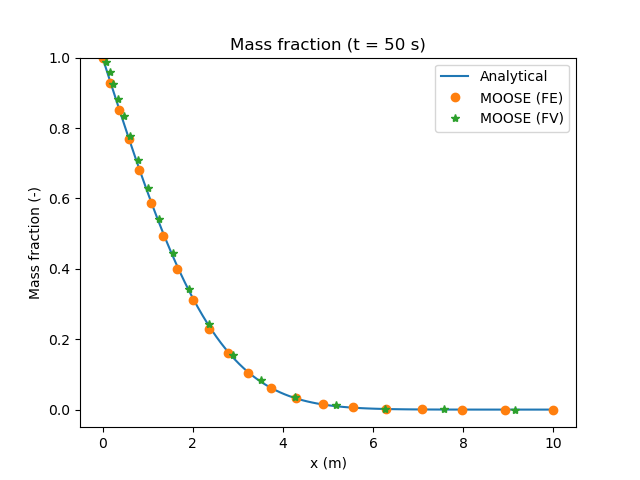
\includegraphics[width=12cm]{diffusion_fig.pdf}
\caption{Mass fraction profile from diffusion only}
\label{fig:diff}
\end{figure}

\chapter{Hydrodynamic dispersion}

The MOOSE results are compared to known analytical solutions for simple problems in order to vertify that the MOOSE implementation is working properly. For a simple 1D model with no diffusion and constant velocity $v$, an analytical solution for the mass fraction profile is given by Javendel et al. (1984)\footnote{Javandel, I, Doughty, C, Tsang, C-f, Groundwater Transport, Handbook of Mathematical Models, AGU, 1984},
\begin{align}
C(x, t) = & C_0 \left\{ \frac{1}{2} \erfc\left(\frac{x- v t}{2 \sqrt{D t}}\right) + \left(\frac{v^2 t}{\pi D}\right)^{1/2}
\exp \left(- \frac{\left[x - vt\right]^2}{4 D T}\right)\right. \nonumber \\
& - \left. \frac{1}{2} \left(1 + \frac{v x}{D} + \frac{v^2 t}{D} \right) \exp\left(\frac{v x}{D}\right) \erfc\left(\frac{x+v t}{2 \sqrt{D T}}\right)\right\},
\end{align}
where all parameters have been previously defined.

The comparison between the automatic test problem \emph{disp01} and the analytical solution is presented in Figure \ref{fig:disp}. The MOOSE results do not coincide with the analytical solution near the top and bottom of the concentration front due to numerical dispersion. If the number of elements in the mesh is increased and the time step size is reduced, numerical dispersion is reduced and a much closer fit to the analytical solution is obtained, see Figure \ref{fig:dispheavy}. This second test is marked as heavy as it takes approximately 5 seconds to run, but is available in the automatic test suite.
\begin{figure}[htb]
\centering
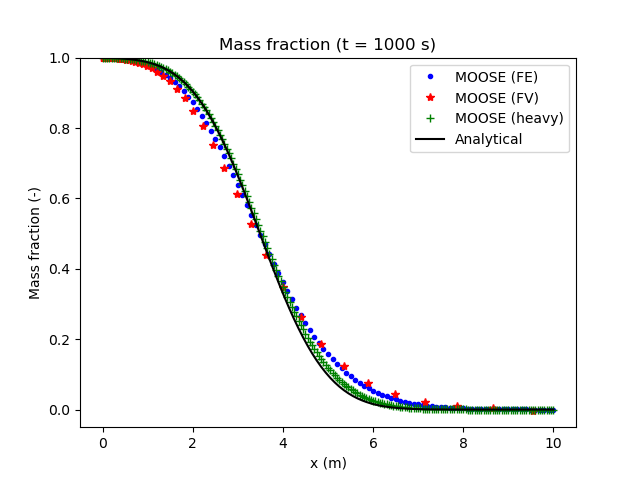
\includegraphics[width=12cm]{dispersion_fig.pdf}
\caption{Mass fraction profile from hydrodynamic dispersion only}
\label{fig:disp}
\end{figure}

\begin{figure}[htb]
\centering
\includegraphics[width=12cm]{dispersion_heavy_fig.pdf}
\caption{Mass fraction profile from hydrodynamic dispersion only using a more refined grid and smaller time steps}
\label{fig:dispheavy}
\end{figure}



\end{document}
